
\section{引言/Introduction}

Edholm带宽定律指出,无线通信的带宽需求每隔18个月翻一倍,预计2030年无线传输的峰值速率将超过Tbit/s量级,日渐趋近于有线传输的容量水平。如今5G 使用非常高的毫米波频段,但是 6G 计划使用 100 GHz以上的更高频率,以便满足相较于 5G NR 而言更高的数据传输速率和更低的延迟需求。
如图所示,太赫兹频段(0.1-10THz)介于微波与红外之间,具有丰富的频谱与带宽资源,能够支持实现Tbit/s量
级的传输速率。

\begin{figure}[htbp]
	\centering
	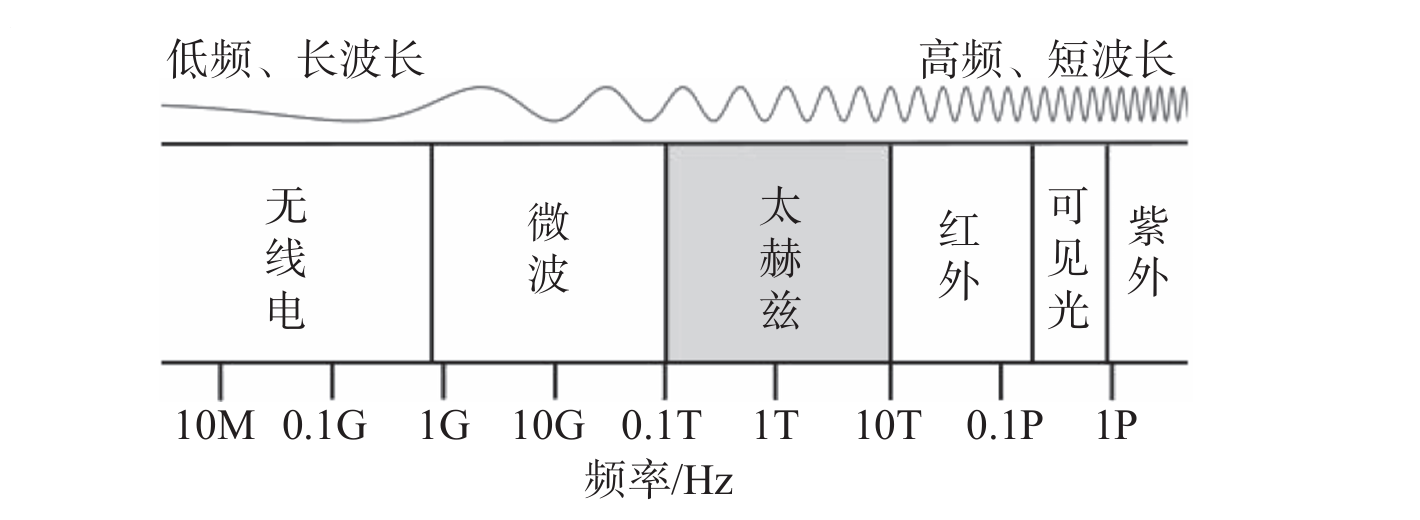
\includegraphics[width=0.6\textwidth]{img/img1.png} % 图片文件名,不需要加扩展名
	\caption{太赫兹频段示意图 \cite{chen2019artificial}}
	\label{fig:example}
\end{figure}

因此,太赫兹通信是 6G 的技术要素之一,其他技术要素包括通信感知一体化 (ISAC)(也称联合通信和传感 (JCAS))、AI 和 ML 以及可重构智能超表面 (RIS)。6G 通信还将使用当前 5G 网络支持的所有频率,例如毫米波频率和传统的 Sub-8 GHz 频段。\\

本文研究了太赫兹成像和太赫兹无线通信技术,重点介绍了这些领域的主要成就和最新进展,确定了它们的相似性和差异,以便更好地理解和探索这些技术。此外,本文还讨论了这两种技术的整合,强调了面临的挑战,并提出了未来的发展方向。本文的其余部分安排如下:第2节介绍了太赫兹技术的基础知识,重点是辐射特性和信号生成;第3节回顾了太赫兹成像技术从过去到现在的发展,包括其主要方法、成就和挑战;第4,5节讨论了太赫兹无线通信,包括其设计架构、技术现状、主要挑战和可能的解决方案,其中重点叙述了基于微型石墨烯贴片的天线,该天线在太赫兹频域具有谐振功能;第6节对两种技术进行了比较,讨论了两种技术整合的可能性,并给出了结论和未来的展望。







